
    \documentclass[journal,twoside]{IEEEtran}
    \usepackage{cite}
\usepackage[pdftex]{graphicx}
\graphicspath{{./voltagesag/}}
\DeclareGraphicsExtensions{.png,.jpeg,.pdf}
\usepackage{amsmath}
\usepackage{algorithmic}
\usepackage{array}
\usepackage{url}
    \begin{document}
    \setcounter{page}{37}
    \title{Voltage sag Detection and Compensation (Single phase) Using Dynamic Voltage Restorer}
    \author{\IEEEauthorblockN{Bibek ~K.~C, Bibek~Pandey, Pawan~Shah and~Saroj~Sapkota*}\\
    \IEEEauthorblockA{Department of Electrical Engineering, Institute of Engineering, Tribhuvan University, Pulchowk, Lalitpur, Nepal \\
    *Email: sarojsapkota338@gmail.com}
    }

\markboth{Zerone Scholar,~Vol.~1, No.~1, November~2016}%
{K.C.\MakeLowercase{\textit{et al.}}: Dynamic Voltage Restorer.}
    \maketitle
	\begin{abstract}
Dynamic Voltage Restorer is a custom
power device used in electrical distribution system for
power quality improvement. The main application of it
is for voltage compensation of sensitive loads against
voltage disturbances such as voltage sag and voltage swell
in distribution lines. It is a series connected device and is
able to compensate voltage sag and voltage swell by
injecting a voltage with the help of series injection
transformer. Conventionally, Dynamic Voltage Restorer consists of an energy
storage device which supplies the required power over the
limited duration of the sags through a inverter.
	\end{abstract}
	\begin{IEEEkeywords}
Voltage Fluctuation, Voltage Restore, DVR
	\end{IEEEkeywords}
	\section{Introduction}
\IEEEPARstart{V}{}oltage sags are a common occurrence in modern power systems. Sags are often caused by normal power system operation during switching or the operation of protective devices in the system, such as re-closers. In other cases, natural and man-made events such as faults or insulator
flashovers due to animals, trees, wind, automobile accidents, and lightning may cause a temporary magnitude reduction of the voltage on one or more phases.

\bigskip
Voltage, sag and swells are considered to be one of the most severe disturbances to the sensitive loads. Dynamic Voltage Restorer (DVR) is a power electronics device which protects sensitive loads from disturbances in the power supply. It ensures high power quality for sensitive loads. The DVR has become popular as a cost effective solution for the protection of sensitive loads from voltage sag and voltage swell. It injects voltage in series and synchronism with the grid supply voltage in order to compensate for voltage sag and voltage swell. DVR is connected in series with line through injection transformer. Fig.~\ref{f1} shows the single phase DVR, which is connected in series with load. When any fault occurs or heavy load is switched on voltage sag occurs across the sensitive load.
\begin{figure}[!ht]
\centering
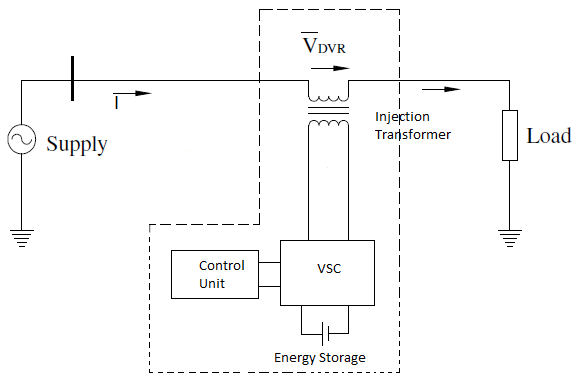
\includegraphics[width=3in]{1}
\caption{Dynamic Voltage Restorer Schemaic Diagram}
\label{f1}
\end{figure}
\bigskip
In order to mitigate the voltage sag problem, DVR is used. During the period of voltage sag DVR injects the voltage so as to restore the load voltage to its normal value. The voltage can be supplied by using energy
storage element in the DVR through the inverter controlled with suitable control logic. Various energy storage devices like batteries, capacitors, etc. are used in DVR. Generally, Three voltage injection techniques are popularly used in DVR, to restore the phase and magnitude of voltage across the sensitive load. These are pre-sag voltage compensation, energy optimization technique and in-phase voltage injection technique.



\section{Proposed Scheme}
This paper presents pre-sag compensation method with missing voltage technique to determine the required voltage to be injected in the system by the DVR. In this method, instantaneous pre-fault voltage and instantaneous post-fault voltage is compared and error voltage is generated which provide required missing voltage magnitude and phase angle. This missing voltage is used to generate gate signal to operate the inverter through which required missing voltage is injected to the system through injection transformer. 

\bigskip
As shown in Fig.1, control unit continuously monitor supply voltage and when disturbance occurs it generates error signal by comparing it with reference voltage or pre-fault or pre-sag voltage which is then fed to voltage source controller (VSC) which generate required missing voltage to be injected as $V_{dvr}(t)$ so that voltage at load remain as pre-fault or pre-sag voltage.

\bigskip
If $V_{pre-sag}(t)$ is the instantaneous voltage across the load which is locked in magnitude, frequency and phase angle to the pre-event voltage and if $V_{sag}(t)$ is disturbed waveform, then the missing voltage $V_{dvr} (t)$ at any instant is the difference:\\
\begin{equation}
V_{dvr}(t) =V_{pre-sag}(t)-V_{sag}(t)
\end{equation}
\\Mathematically,\\
\begin{equation}
V_{pre-sag}(t)=A*sin(\omega t-\phi _{1})
\end{equation}
\begin{equation}
V_{sag}(t)=B*sin(\omega t-\phi _{2})
\end{equation}
where, A,B are the amplitudes of the $\phi _1$and $\phi _2$  are the phase angle of pre-sag and after sag voltage respectively. If we assume same frequency for both, then missing voltage $V_{dvr}(t)$ can be calculated as:\\
\begin{equation}
V_{dvr}(t)=Rsin(\omega t - \psi)
\end{equation}
\\where,\\
\begin{equation}
R=\sqrt{A^2+B^2-2ABcos(\phi _1-\phi _2)}
\end{equation}


\bigskip
\begin{equation}
tan{ \psi }=\frac{Asin{\phi _1}-Bsin{\phi _2}}{Acos{\phi _1}-Bcos{\phi _2}}
\end{equation}

\bigskip

Here, R and $tan(\psi)$ are the required amplitude and phase angle to recover the to the pre-fault or pre-sag condition. There are many methods of injecting voltage through DVR which are as:
\begin{itemize}

\item{1.} pre-sag compensation method
\item{2.} in-phase compensation method
\item{3.} in-phase advance compensation method
\item{4.} voltage tolerance method with minimum energy
injection
\end{itemize}
In this method of missing voltage technique pre-sag compensation method is used in which supply voltage is monitor continuously and if any disturbance is detected,it will inject the difference voltage between the sag and pre-fault voltage so that load voltage re-stored back to pre-fault voltage. Both magnitude and phase angle can be compensated by this technique. 
If $\phi _1 = 0 $and $\phi _2 = 0$ in equation (2) and (3) then
Equation (4) becomes:

\begin{equation}
V_{dvr}(t)= Rsin(\omega t –\psi) = R sin(\omega t )
\end{equation}


The result for A = 80 and B = 60 is shown in Matlab
simulation and results section.
	

\section{Modelling of Proposed Scheme}

Peak detection method:
Assume that the input voltage v(t) is given by:
\begin{equation}
v(t) = V_psin(\omega t)
\end{equation}
Where $V_p$ is the peak value of the input voltage. If v(t) is
sent through a $90 \deg$ phase shift circuit, then v'(t) is
obtained as,
\begin{equation}
v'(t) =V_p sin(\omega t +\frac{\pi}{2} )=V_p cos(wt)
\end{equation}

The two signals, v(t) and v'(t) are a pair of orthogonal
functions. If they are sent through the two separate
multipliers and squared, the following two equations can
be obtained:

\begin{align}
V_{01}(t)=KV_p^2sin^2(\omega t)\\
V_{02}(t)=KV_p^2cos^2(\omega t)
\end{align}
Where, K is the multiplication factor of the multipliers.
Due to the characteristic of orthogonal functions $V_{01}(t)$
and $V_{02}(t)$, it is easy to obtain the square of the input
voltage peak value by adding equation (10) and (11).

\begin{align}
V_{0a}(t) = V_{01}(t)+ V_{02}(t)\notag\\
\qquad = KV_p^2 (sin^2(\omega t) + cos^2 (\omega t) )\notag\\
\qquad = KV_p^2
\end{align}
In order to measure the peak value, the signal v 0a (t) is
fed to a square root circuit. Then the output of the square
root circuit is:

Where $K_1$ is the multiplication factor of the square root
circuit. If the multiplication factors of the multiplier and
the square root circuit are selected properly, the value of
constant $K_1$ can be set to 1. The output voltage of the
detector is equal to the peak value of the input voltage.
Because the detector is based on the concept of an
orthogonal function pair, it is called \lq orthogonal
detector\rq.

Fig.~\ref{f2} shows the block diagram of voltage measurement
using the peak detection method.


\begin{figure}[!ht]
\centering
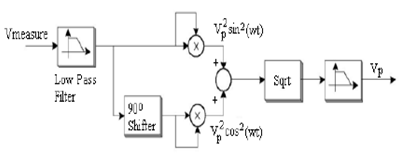
\includegraphics[width=3in]{2}
\caption{Peak Detection Method}
\label{f2}
\end{figure}


$V_{measure}$ shown in Fig.~\ref{f2} a represent the single phase line
to neutral voltage. This voltage is shifted by 90o using
90o shifter to obtain cosine value. Assuming the line
frequency as 50Hz, the 90o shifted value can be obtained
by either an analog circuit or by digital signal
processing. Both components of voltage are squared and
summed to yield $V_p^2$ . Peak value is then obtained by
squaring root of $V_p^2$ . The significant advantage of peak
value evaluation compared to others method is that it
only needs single phase values.

The output value of peak detection block is compared
with the input voltage as shown in Fig.~\ref{f3} The comparison
verifies the ability of method in detecting the peak value
of the input signal in the least possible time.
\begin{figure}[!ht]
\centering
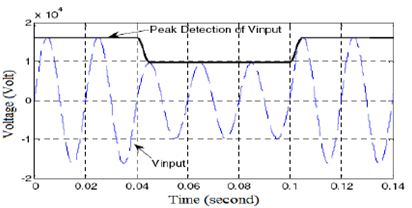
\includegraphics[width=3in]{3}
\caption{Peak Detection Signal and $V_input$ signal}
\label{f3}
\end{figure}

	\section{Matlab Simulations and Results}

MATLAB block diagram for voltage sag detection and
compensation is shown Fig~\ref{f4}.
\begin{figure}[!ht]
\centering
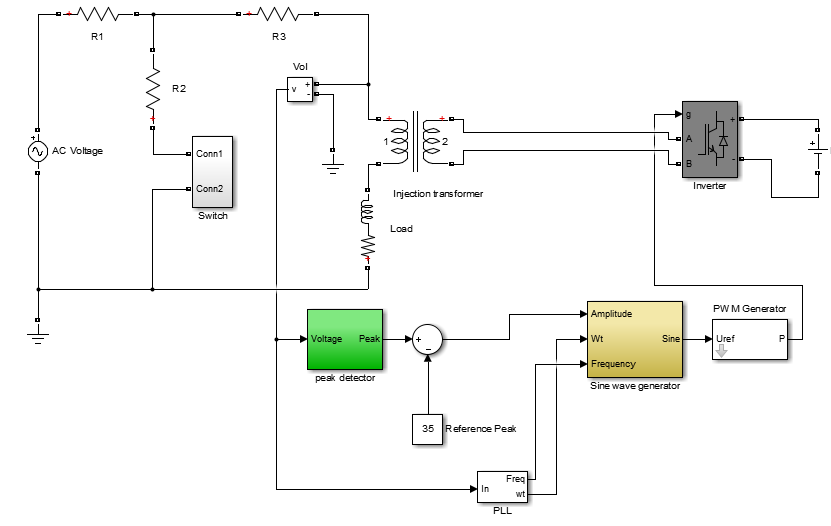
\includegraphics[width=3in]{4}
\caption{Dynamic Voltage Restorer Schemaic Diagram}
\label{f4}
\end{figure}


In the simulation, the values of A, B, $\phi _1$ and $\phi _2$ are
taken as 30, 15, 0, and 0 respectively, which gives:
$V_{dvr}(t)= Rsin(\omega t )$

Here, $\psi$ = 0 and the wave is sinusoidal in nature.

The resulting waveform and plot of rms values of the
voltage without DVR are shown in Fig~\ref{f5},~\ref{f6}
respectively.

\begin{figure}[!ht]
\centering
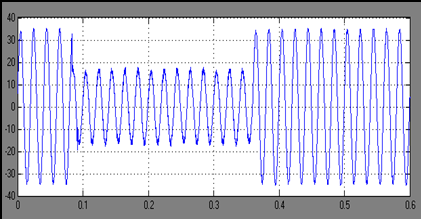
\includegraphics[width=3in]{5}
\caption{Voltage sag of duration of 0.25 sec in load voltage
in absence of DVR}
\label{f5}
\end{figure}


\begin{figure}[!ht]
\centering
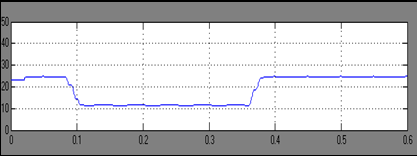
\includegraphics[width=3in]{6}
\caption{Plot of RMS value of voltage for a sag duration of
0.25 sec in absence of DVR}
\label{f6}
\end{figure}

When the DVR is incorporated in the system missing
voltage of peak 15V is achieved which is shown in Fig.~\ref{f7}
\begin{figure}[!ht]
\centering
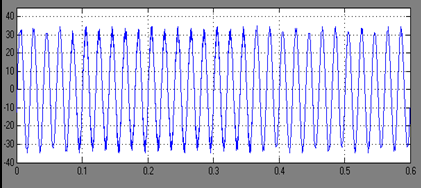
\includegraphics[width=3in]{7}
\caption{Load voltage during disturbance in presence of DVR}
\label{f7}
\end{figure}
Fig.~\ref{f8} shows the plot of RMS value of load voltage in
presence of DVR.

\begin{figure}[!ht]
\centering
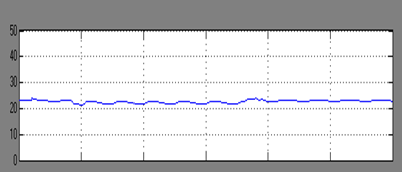
\includegraphics[width=3in]{8}
\caption{Plot of rms value of load voltage in presence of DVR}
\label{f8}
\end{figure}


From the above simulation results, it is clear that voltage
sag problem can be eliminated with the help of DVR. In
the simulation result, voltage sag of duration 0.25 sec is
removed with the help of DVR.

	\section{Conclusion}

DVR with missing voltage technique can eliminate the
voltage sag problem with fast response. In this paper, it
has only considered sinusoidal sag. But in real case, non-
sinusoidal sag may occur. This work can further extended
for compensation of non-sinusoidal sag.


\begin{thebibliography}{9}

    \bibitem{Bollen1999} 
        M.H.J. Bollen, \emph{Understanding Power Quality
        Problems: Voltage Sags and Interruptions}, New
        York:IEEE Press, Vol. 1, 1999.

    \bibitem{Tuna1998} 
        N.S. Tuna boylu, E.R. Collins, Jr., P.R.Chaney,
        \emph{Voltage disturbance evaluation using the missing
        voltage technique}, International Conference on
        Harmonics and Quality of Power, Vol. 1, pp. 577-
        582,1998.

    \bibitem{Deckmann2002} 
        S.M. Deckmann, A.A. Ferreira, \emph{About Voltage Sags
        and Swell Analysis},IEEE, pp. 144-148, 2002.

    \bibitem{Bollen1996} 
        M. H. J. Bollen, P. Wang, N. Jenkins, \emph{Analysis and
        consequences of the phase jump associated with a
        voltage sag}, Power Systems Computation Conf.,
        August 1996, Dresden, Germany.

\end{thebibliography}


\newpage

\begin{IEEEbiography}[{
\includegraphics[width=1in,height=1.25in,clip,keepaspectratio]{bp}}]{Bibek Pandey}
\end{IEEEbiography}

\begin{IEEEbiography}[{
\includegraphics[width=1in,height=1.25in,clip,keepaspectratio]{bk}}]{Bibek K.C.}
\end{IEEEbiography}
\newpage
\begin{IEEEbiography}[{
\includegraphics[width=1in,height=1.25in,clip,keepaspectratio]{pks}}]{Pawan Kumar Shah}
\end{IEEEbiography}

\begin{IEEEbiography}[{
\includegraphics[width=1in,height=1.25in,clip,keepaspectratio]{ss}}]{Saroj Sapkota}
\end{IEEEbiography}

\end{document}

